\documentclass[a4paper,oneside,article,11pt]{memoir}
\usepackage[english]{babel}
\usepackage[utf8]{inputenc}
\usepackage{amsmath,amssymb,amsthm}

% This font looks so good.
\usepackage[sc]{mathpazo}

% Typesetting pseudo-code
\usepackage{algorithm}
\usepackage{algorithmic}
\usepackage{multirow}
% Code comments like [CLRS]
\renewcommand{\algorithmiccomment}[1]{\makebox[5cm][l]{$\triangleright$ \textit{#1}}}
\usepackage{framed,graphicx,xcolor}
\usepackage[font={small,it}]{caption}
\usepackage{listings}
\usepackage{units}

% Relative references
\usepackage{varioref}

\usepackage{hyperref}

\bibliographystyle{plain}

\title{Advanced Data Structures \\ Project 1 - Fibonacci heaps}
\author{Peter Gabrielsen 20114179 \\
Christoffer Hansen 20114637}
\newcounter{qcounter}
\begin{document}

\begin{titlingpage}
\clearpage

\maketitle
\thispagestyle{empty}

\begin{abstract}
ABSTRACT HERE
\\
\\
\\
The code can be found at: \\\url{CODE HERE}.
\end{abstract}
\end{titlingpage}

\pagebreak

\tableofcontents

\pagebreak

\chapter{Introduction}
INTRO

\chapter{Implementation}
Talk about implementing fibonacci heap and binary heap

Implement
the Fibonnacci Heaps of Fredman and Tarjan,
the binary heaps of Williams (Algorithm 232, CACM 21(4), 1964).
As a minimum the following opeartions should be supported: MakeHeap, FindMin, Insert, DeleteMin, and DecreaseKey.

\chapter{Experiments}
Design and perform experiments where you try to measure the running time and number of comparisons of the operations for both priority queue implementations.

%TODO compiling using O2 makes bh better than fh but not in worst case MSP

\chapter{Theory}
Argue about the worst-case (as opposed to amortized) time bounds for each of the operations of Fibonnacci Heaps and binary heaps.

\chapter{Dijkstra's algorithm}
In this section we introduce families of graphs that we believe makes Dijkstra's algorithm perform many respectively few \texttt{DecreaseKey} operations. It is obvious that the number of \texttt{DecreaseKey} operations is an exact measure of the number of edges we have to relax.

\section{Few relaxations}
Since Dijkstra's algorithm finds shortest paths from the source $s$ to all vertices in the graph, we have to relax at least one ingoing edge for all other vertices. We therefore conclude that the lower bound for relaxing edges must be $\vert V \vert -1$. If not, the graph would contain unvisited vertices. Having a chain of vertices with \textit{weight} 0 on all edges causes Dijkstra to \textit{relax} each edge exactly once, giving us a graph with the desired property. It is clear that not additional (positive weighted) edges will be relaxed. For a graphical representation of the described class of graphs, please to figure~\ref{figure:graph_chain}.

\begin{figure}
\centering
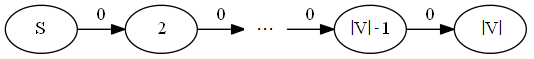
\includegraphics[scale=1]{../figures/graph_chain.png}
\caption{Chain of $\vert V \vert$ nodes with edge weight 0.}
\label{figure:graph_chain}
\end{figure}

\section{Many relaxations}
We consider an analysis of Dijkstra's algorithm using the fact that our implementation makes use of a priority queue $Q$. Since each vertex is removed from $Q$ exactly once, and the adjacency list of each vertex is scanned exactly once, it is clear that we can at most relax all edges exactly once.
In other words we need to consider graphs that makes Dijkstra's algorithm perform $\vert E \vert$ \texttt{DecreaseKey} operations in order to reach the upper bound.

We present two candidates of classes of graphs with the above mentioned property. The first proposal makes use of negative weights. Since we are not introducing negative cycles, Dijkstra's algorithm would still be able run, but as we allow for previously marked nodes to be reinserted into the priority queue, we cannot rely on the asymptotic time bound. The second proposal uses only positive edge weights, and can therefore be compared against the asymptotic analysis.

\begin{figure}
\centering
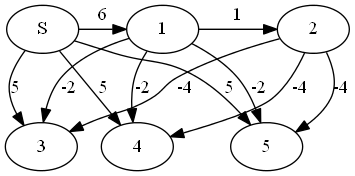
\includegraphics[scale=0.8]{../figures/graph_neg_weights.png}
\caption{}
\label{figure:graph_neg_weights}
\end{figure}

\begin{figure}
\centering
\centerline {
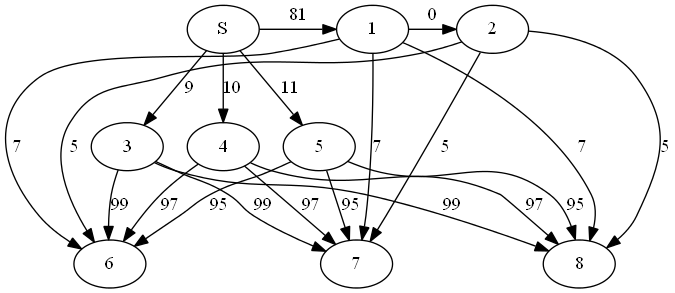
\includegraphics[scale=0.5]{../figures/graph_positive_weights.png}
}
\caption{}
\label{figure:graph_neg_weights}
\end{figure}

\chapter{Experiments on Dijkstra's}
Perform experiments on your implementation of Dijkstra's algorithm - in particular, try to observe if the version using Fibonacci heaps achieves an improved performance because of the amortized O(1) time DecreaseKey operation.

\section{System configuration and methodology}
\label{sec:machine}
The experiments were performed on a machine with a Intel i5 @ 2.5GHz (Ivy Bridge) with 128K bytes of L1 cache, 512K bytes of L2 and 3072K bytes of L3 cache. The machine had 4.2GB ram and ran Ubuntu 14.04 with kernel version 3.16.0-30. The internal mechanical disc was a 1TB Samsung SpinPoint M8 SATA II 2.5'' laptop hard drive with 8MB cache running at 5400 RPM with a seek time of 12.0ms.

The running time was measured using the built in \texttt{high\_resolution\_clock} in the \texttt{chrono} library. This measures the wall clock. It is the clock in \texttt{c++} with the highest precision, i.e. the shortest tick period.

The code is compiled with \texttt{g++ 4.8.2} with the \texttt{c++11} standard enabled and no optimization level.

Correctness was tested on random 32-bit integers generated uniformly in the integer range [0,...,1000] using the Mersenne Twister 19937 from the \texttt{random} library.

Running time was on random 32-bit integers generated using the system call \textit{head -c 64GB $<$dev/urandom $>$test64gb}.

All experiments were done using \textit{bstream} with a buffer size of 2048 integers (8192 bytes).

Each experiment was executed 5 times and the average was used as the result.


\bibliography{references}

\end{document}


